\documentclass[border=6pt,tikz]{standalone}
\usepackage{tikz}
\usepackage{amsmath,amssymb}
\usetikzlibrary{arrows.meta,positioning,fit,backgrounds,calc,shapes.geometric,decorations.pathreplacing,patterns}
\definecolor{ink}{HTML}{1B2430}
\definecolor{muted}{HTML}{6B7785}
\definecolor{accent}{HTML}{2F6FB5}
\definecolor{accent2}{HTML}{C1611F}
\definecolor{good}{HTML}{2E7D5B}
\definecolor{soft}{HTML}{EDF2F7}
\definecolor{soft2}{HTML}{FBEDE2}
\definecolor{soft3}{HTML}{E6F0E9}
\tikzset{
  box/.style={draw=ink,line width=.7pt,rounded corners=2pt,fill=soft,inner sep=4pt,align=center,font=\sffamily\small},
  boxa/.style={box,fill=soft2},
  boxb/.style={box,fill=soft3},
  plain/.style={align=center,font=\sffamily\small,text=ink},
  tiny/.style={align=center,font=\sffamily\scriptsize,text=muted},
  ar/.style={-{Stealth[length=2.4mm]},draw=ink,line width=.7pt},
  arm/.style={-{Stealth[length=2.4mm]},draw=muted,line width=.6pt,dashed},
  nd/.style={circle,draw=ink,line width=.7pt,fill=white,minimum size=7mm,inner sep=0pt,font=\sffamily\scriptsize},
  ndf/.style={nd,fill=soft},
  ndt/.style={nd,fill=soft2},
}

\begin{document}
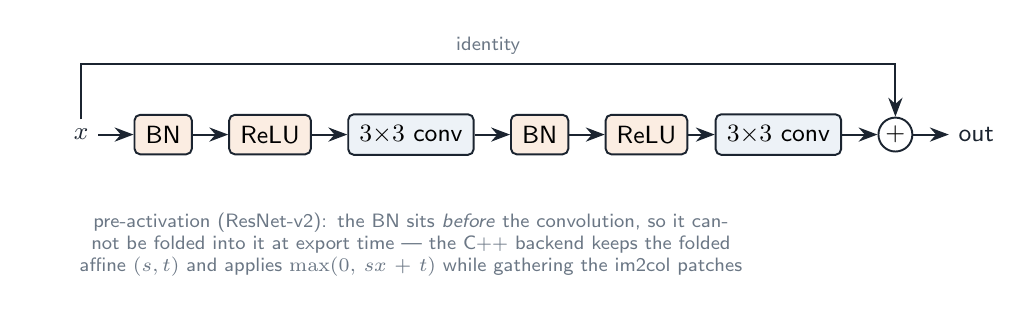
\begin{tikzpicture}[node distance=4.5mm]
  \node[plain] (x) {$x$};
  \node[boxa,right=of x] (bn1) {BN};
  \node[boxa,right=of bn1] (r1) {ReLU};
  \node[box,right=of r1] (c1) {$3{\times}3$ conv};
  \node[boxa,right=of c1] (bn2) {BN};
  \node[boxa,right=of bn2] (r2) {ReLU};
  \node[box,right=of c1,xshift=26mm] (c2) {$3{\times}3$ conv};
  \node[circle,draw=ink,line width=.7pt,right=of c2,inner sep=1pt,font=\small] (add) {$+$};
  \node[plain,right=of add] (out) {out};
  \draw[ar] (x) -- (bn1); \draw[ar] (bn1) -- (r1); \draw[ar] (r1) -- (c1);
  \draw[ar] (c1) -- (bn2); \draw[ar] (bn2) -- (r2); \draw[ar] (r2) -- (c2);
  \draw[ar] (c2) -- (add); \draw[ar] (add) -- (out);
  \draw[ar] (x.north) -- ++(0,7mm) -| node[tiny,pos=.25,above]{identity} (add.north);
  \node[tiny,below=6mm of c1,text width=95mm] {pre-activation (ResNet-v2): the BN sits \emph{before} the convolution, so it
    cannot be folded into it at export time --- the C++ backend keeps the folded affine
    $(s,t)$ and applies $\max(0,\,s x+t)$ while gathering the im2col patches};
\end{tikzpicture}
\end{document}
